\documentclass[12pt]{article}
\usepackage[T1, T2A]{fontenc}
\usepackage[utf8]{inputenc}
\usepackage[russian]{babel}
\usepackage{hyperref}
\usepackage{datetime}
\usepackage{amsmath}
\usepackage{amsfonts}
\usepackage{tikz}
\graphicspath{ {./Images/} }

\usepackage{pgfplots}
\pgfplotsset{compat=newest}
\usepgfplotslibrary{fillbetween}
\usetikzlibrary{calc}
\usetikzlibrary{shapes.geometric}


\usepackage[14pt]{extsizes} % для того чтобы задать нестандартный 14-ый размер шрифта
\usepackage[utf8]{inputenc}
\usepackage[russian]{babel} % поддержка русского языка
\usepackage{amsmath}  %  математические символы
\usepackage[left=20mm, top=15mm, right=15mm, bottom=30mm, footskip=15mm]{geometry} % настройки полей документа
\usepackage{indentfirst} % по умалчанию убирается отступ у первого абзаца в секции, это отменяет это.
\usepackage{paralist} % добавить компактные списки (compactitem, compactenum, compactdesc)

\usepackage{fancyvrb}
\usepackage{framed}

\usepackage{float}
\floatstyle{ruled}
\newfloat{termfloat}{thp}{lop}
\floatname{termfloat}{Снимок экрана}



\begin{document}
% \maketitle
\begin{titlepage}

	\begin{center}
		\hfill \break
		\textbf{
			\large{РОССИЙСКИЙ УНИВЕРСИТЕТ ДРУЖБЫ НАРОДОВ}\\
			\normalsize{Факультет физико-математических и естественных наук}\\
			\normalsize{Кафедра прикладной информатики и теории вероятностей}\\
		}
		\vspace*{\fill}
		\Large{\textbf{Индивидуальное домашнее задание \textnumero 1}}
		\\
		\underline{\textit{\normalsize{Дисциплина: Теория вероятностей и математическая статистика}}}
		\vspace*{\fill}

	\end{center}

	\begin{flushright}
		Студент: \underline{Григорий Матюхин}\\ \vspace{0.5cm}
		Группа: \underline{НПИбд-01-21}
	\end{flushright}


	\begin{center} \textbf{МОСКВА} \\ 2021 г. \end{center}
	\thispagestyle{empty} % выключаем отображение номера для этой страницы

\end{titlepage}
\newpage
\tableofcontents
\newpage

\section*{Задание \textnumero1.}
\addcontentsline{toc}{section}{Задание \textnumero1.}
Найдите вероятность того, что произведение двух последних цифр номера автомобиля:
\begin{enumerate}
	\item Равно $n$;
	\item Больше $n$;
	\item Меньше $n$;
	\item Заключено в промежутке $[n_1; n_2]$.
\end{enumerate}
$n = 10; n_1 = 15; n_2 = 45$

\subsection*{Решение}
\begin{enumerate}
	\item Равно 10:
	      \begin{gather*}
		      \Omega = \{\omega_{ij}; i, j = \overline{0, 9}\}, |\Omega| = 100 \\
		      A = \{\omega_{25}, \omega_{52}\}, |A| = 2 \\
		      P(A) = \frac{|A|}{|\Omega|} \\
		      P(A) = \frac{2}{100} = 0.02
	      \end{gather*}
	\item Больше 10:
	      \begin{gather*}
		      B = \{\omega_{ij}; \omega_{2a}; \omega_{b2}; \omega_{3c}; \omega_{d3}; \} \\
		      i, j, c, d = \overline{4, 9}; a, b = \overline{6, 9}; \\
		      |B| = 56
		      P(B) = \frac{|B|}{|\Omega|} \\
		      P(B) = \frac{56}{100} = 0.56
	      \end{gather*}
	\item Меньше 10:
	      \begin{gather*}
		      C = \Omega \setminus (A \cup B) \\
		      P(C) = 1 - \frac{1}{50} - \frac{28}{50} = \frac{42}{100} = 0.42
	      \end{gather*}
	\item Заключено в промежутке $[15; 45]$:
	      \begin{gather*}
		      D = \{ \\
		      \omega_{28}; \omega_{29}; \\
		      \omega_{35}; \omega_{36}; \omega_{37}; \omega_{38}; \omega_{39}; \\
		      \omega_{44}; \omega_{45}; \omega_{46}; \omega_{47}; \omega_{48}; \omega_{49}; \\
		      \omega_{53}; \omega_{54}; \omega_{55}; \omega_{56}; \omega_{57}; \omega_{58}; \omega_{59}; \\
		      \omega_{63}; \omega_{64}; \omega_{65}; \omega_{66}; \omega_{67}; \\
		      \omega_{73}; \omega_{74}; \omega_{75}; \omega_{76}; \\
		      \omega_{82}; \omega_{83}; \omega_{84}; \omega_{85}; \\
		      \omega_{92}; \omega_{93}; \omega_{94}; \omega_{95} \\
		      \}, |D| = 37 \\
		      P(D) = \frac{|D|}{|\Omega|} = \frac{37}{100} = 0.37
	      \end{gather*}
\end{enumerate}

\subsection*{Ответ}
\begin{enumerate}
	\item 0.02
	\item 0.56
	\item 0.42
	\item 0.37
\end{enumerate}

\newpage
\section*{Задание \textnumero2.}
\addcontentsline{toc}{section}{Задание \textnumero2.}
В треугольник с вершинами в точках $(a_1;b_1)$, $(a_2;b_2)$ и $(a_3; b_3)$ в соответствии с принципом геометрической вероятности бросается точка.
Обозначим через $\xi$ и $\eta$ координаты этой точки.
Вычислите вероятность того, что квадратное уравнение $x^2 + 2(\xi - c)x + d\eta + f = 0$ будет иметь действительные корни. \\
$(a_1;b_1)=(1;3); (a_2;b_2)=(0;1); (a_3;b_4)=(3;0); c = 3; d = -2; f = 4$

\subsection*{Решение}
\begin{gather*}
	x^2 + 2(\xi - 3)x - 2\eta + 4 = 0 \\
	D = (2(\xi - 3))^2 - 4(4 - 2\eta) = 4\xi^2 - 24\xi + 20 + 8\eta \\
\end{gather*}
Чтобы данное уравнение имело ревальные корни дискриминант $D$ должен быть больше или равен 0
\begin{gather*}
	4\xi^2 - 24\xi + 20 + 8\eta \geq 0 \\
	\eta \geq -\frac{1}{2} \xi^2 + 2\xi - \frac{3}{2}
\end{gather*}

\begin{tikzpicture}
	\begin{axis}[
			axis lines = middle,
			xlabel = {$x$},
			ylabel = {$y$},
			xmin=0, xmax=4,
			ymin=0, ymax=4]

		% Curve 
		\addplot [name path = A,
			-latex,
			domain = 0:4,
			samples = 1000] {-1/2 * x^2 + 3*x - 3/2}
		node [very near end, right] {};

		% Top fill bound
		\addplot [name path = B,
			domain = 0:4] {5}
		node [pos=1, above] {$y = 4$};

		% Triangle 
		% Top left
		\addplot [name path = T1,
			domain = 0:1] {2*x + 1}
		node [pos=1, above] {};

		% Top right
		\addplot [name path = T2,
			domain = 1:4] {-3/2 * x + 9/2}
		node [pos=1, above] {};

		% Bottom
		\addplot [name path = T3,
			domain = 0:4] {-1/3 * x + 1}
		node [pos=1, above] {};


		\path[%draw=magenta,thick,->,
		intersection segments={
		of=A and T2,
		sequence={R1--L1[reverse]}
		}, name path=R];

		\path[%draw=blue,thick,->,
		intersection segments={
		of=T3 and R,
		sequence={R1--L1[reverse]}
		}, name path=RB];

		\path[%draw=red,thick,->,
			fill=orange,
			intersection segments={
					of=RB and T1,
					sequence={L2--R2}
				}];

		\path[name intersections={of=A and T2,by=N}];
		\draw (N) node[above=.5em] {A} circle[radius=2pt];

		\path[name intersections={of=A and T3,by=M}];
		\draw (M) node[above=.5em] {B} circle[radius=2pt];

	\end{axis}
\end{tikzpicture}

Найдем уравнения сторон треугольника:
\begin{gather*}
	y_1 = 2x + 1 \textup{ --- левая сторона} \\
	y_2 = -\frac{3}{2}x + \frac{9}{2} \textup{ --- правая сторона} \\
	y_3 = -\frac{1}{3}x + 1 \textup{ --- нижняя сторона}
\end{gather*}
Найдем точки $A$ и $B$:
\begin{gather*}
	-\frac{1}{2} x^2 + 2x - \frac{3}{2} = -\frac{3}{2}x + \frac{9}{2} \\
	x_1 = \frac{9}{2} - \frac{\sqrt{33}}{2} = 1.062\\
	x_2 = \frac{9}{2} + \frac{\sqrt{33}}{2} \\
	y = -\frac{3}{2} \left(\frac{9}{2} - \frac{\sqrt{33}}{2}\right) + \frac{9}{2} = 2.058 \\
	A = (1.628; 2.058)
\end{gather*}
Аналогично: $B = (0.861; 0.713)$ \\
Найдем закрашенную площадь:
\begin{gather*}
	S = \int_0^{0.861}\left((2x + 1) - (-\frac{1}{3}x + 1)\right)dx + \\
	+ \int_{0.861}^1\left((2x + 1) - (-\frac{1}{2} x^2 + 3x - \frac{3}{2})\right)dx + \\
	+ \int_1^{1.628}\left(\left(-\frac{3}{2}x + \frac{9}{2}\right) - \left(-\frac{1}{2} x^2 + 3x - \frac{3}{2}\right)\right)dx = \\
	= 0.864875 + 0.278448 + 0.607107 = 1.75043
\end{gather*}
Площадь треугольника:
\begin{gather*}
	\Omega = \int_0^1\left((2x + 1) - \left(-\frac{1}{3}x + 1\right)\right)dx + \\
	+ \int_1^3\left(\left(-\frac{3}{2}x + \frac{9}{2}\right) - \left(-\frac{1}{3}x + 1\right)\right)dx = \\
	= 1.17 + 2.33 = 3.5
\end{gather*}
Тогда вероятность того, что квадратное уравнение $x^2 + 2(\xi - c)x + d\eta + f = 0$ будет иметь действительные корни.
\begin{equation*}
	P = \frac{S}{\Omega} = \frac{1.75043}{3.5} \approx 0.5
\end{equation*}

\subsection*{Ответ}
0.5

\section*{Задание \textnumero3.}
\addcontentsline{toc}{section}{Задание \textnumero3.}
Из двух урн, в каждой из которых находятся $n$ шаров с написанных на них числами от 1 до $n$, наудачу извлекается по одному шару.
Событие $A$ --- сумма чисел, написанных на выбранных шарах, делится на $m$, событие $B$ -- произведение этих чисел больше $k$.
Определите условные вероятности $P(A|B)$ и $P(B|A)$. Являются ли события $A$ и $B$ независимыми? \\
$n = 16; m=7; k = 24$
\subsection*{Решение}
\begin{gather*}
	|A| = 36, |B| = 188, |AB| = 26, |\Omega| = 256 \\
	P(A) \approx 0.14, P(B) \approx 0.73, P(AB) \approx 0.10 \\
	P(A|B) = \frac{P(AB)}{P(B)} \approx 0.14 \\
	P(B|A) = \frac{P(AB)}{P(A)} \approx 0.72
\end{gather*}
Т.к. $P(A) \approx P(A|B)$ и $P(B) \approx P(B|A)$ то события $A$ и $B$ --- независимые.
\subsection*{Ответ}
События $A$ и $B$ --- независимые.

\newpage
\section*{Задание \textnumero4.}
\addcontentsline{toc}{section}{Задание \textnumero4.}
Система надежности состоит из 6 элементов и имеет заданную структурную схему. \\
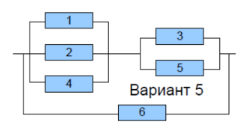
\includegraphics{1.png} \\
События $A_i, i=\overline{1, 6}$, -- отказы элементов за заданный промежуток времени.
\begin{enumerate}
	\item Выразите через события $A_i$ события $A$ и $\overline{A}$, где $A$ — отказ всей системы за заданный промежуток времени.
	\item Считая, что события $A_i$ независимы в совокупности и имеют вероятности $P(A_i)=p_i, i = \overline{1,6}$, вычислите вероятность события $A$.
\end{enumerate}
$p_1 = p_3 = p_5 = 0.3; p_2 = p_4 = p_6 = 0.1$
\subsection*{Решение}
\begin{enumerate}
	\item Выразим $A$ и $\overline{A}$:
	      \begin{gather*}
		      A_{124} = A_1A_2A_3 \\
		      A_{35} = A_3A_5 \\
		      A_{12345} = A_{124} \cup A_{35} \\
		      A = A_{12345} \cap A_6 \Rightarrow \\
		      A = (A_1A_2A_4 \cup A_3A_5) \cap A_6 \\
	      \end{gather*}
	      Отсюда в силу формул де Моргана для события $\overline{A}$ --- безотказной работы устройства получаем выражение
	      \begin{equation*}
		      \overline{A} = \left(\overline{A_1} \cup \overline{A_2} \cup \overline{A_4}\right) \cap \left(\overline{A_3} \cup \overline{A_5}\right) \cup \overline{A_6} \\
	      \end{equation*}
	      где событие $\overline{A_i}, i = \overline{1,6}$ — безотказная работа $i$-гo элемента.
	\item Вычислим вероятность события $A$:
	      \begin{gather*}
		      P(A) = \left(1 - \left[1 - P(A_1)P(A_2)P(A_4)\right]\left[1 - P(A_3)P(A_5)\right]\right)P(A_6) \\
		      P(A) = \left(1 - \left[1 - 0.3 \times 0.1^2\right]\left[1 - 0.3^2\right]\right) \times 0.1 \\
		      P(A) = 0.009273
	      \end{gather*}
\end{enumerate}
\subsection*{Ответ}
\begin{enumerate}
	\item \mbox{}\\
	      $A = (A_1A_2A_4 \cup A_3A_5) \cap A_6$ \\
	      $\overline{A} = \left(\overline{A_1} \cup \overline{A_2} \cup \overline{A_4}\right) \cap \left(\overline{A_3} \cup \overline{A_5}\right) \cup \overline{A_6}$
	\item 0.009273
\end{enumerate}

\section*{Задание \textnumero5.}
\addcontentsline{toc}{section}{Задание \textnumero5.}
В первой урне находятся $n_1$ белых и $m_1$ черных шаров, во второй урне --- $n_2$ белых и $m_2$ черных шаров. Сначала из первой урны во вторую перекладывается наугад $k$ шаров, затем такое же число шаров так же наугад перекладывается из второй урны в первую.
\begin{enumerate}
	\item Определите вероятность того, что после вскрытия первой урны в ней будет столько же белых и черных шаров, сколько было до проведения опыта.
	\item После вскрытия первой урны оказалось, что в ней столько же белых и черных шаров, сколько было до проведения опыта. Вычислите вероятность того, что при этом условии из первой урны во вторую переложили $l$ белых шаров.
\end{enumerate}
$n_1 = 5; m_1 = 1; n_2 = 0; m_2 = 7; k=4; l =4$
\newpage
\subsection*{Решение}
\begin{enumerate}
	\item Используем формулу полной вероятности \\
	      $A$ --- после двух перекладываний туда и обратно состав шаров в первой урне не изменился. \\
	      $H_i, i \in \{3,4\}$ --- из первой урны во вторую переложено $i$ белых шаров. \\
	      Рассчитаем вероятности гипотез:
	      \begin{gather*}
		      P(H_i) = \frac{|H_i|}{|\Omega|} \\
		      |\Omega| = C^k_{n_1 + m_1} = C^4_6\\
		      P(H_3) = \frac{C_{n_1}^3 \times C_{m_1}^1}{|\Omega|} \approx 0.67 \textup{ --- 3 белых шара, 1 черный шар} \\
		      P(H_4) = \frac{C_{n_1}^4 \times C_{m_1}^0}{|\Omega|} \approx 0.33 \textup{ --- 4 белых шара, 0 черных шаров} \\
	      \end{gather*}
	      Рассчитаем условные вероятности: \\
	      $|\Omega_2| = C^4_{11} = 330$ --- во второй урне после перекладывания стало $n_2 + m_2 + k = 0 + 7 + 4 = 11$ шаров.
	      Возвращаем тоже 4. \\
	      $A|H_3$  --- при перекладывании туда и обратно состав шаров в первой урне не изменился при условии, что при первом перекладывании из первой урны во вторую было переложено 3 белый шара и 1 черный и столько же обратно.
	      Количество белых стало $n_2 + 3 = 0 + 3 = 3$, а черных --- $m_2 + 1 = 7 + 1 = 8$.
	      \begin{equation*}
		      P(A|H_3) = \frac{C_3^3 \times C_8^1}{|\Omega_2|} \approx 0.024 \\
	      \end{equation*}
	      $A|H_4$  --- при перекладывании туда и обратно состав шаров в первой урне не изменился при условии, что при первом перекладывании из первой урны во вторую было переложено 3 белый шара и 1 черный и столько же обратно.
	      Количество белых стало $n_2 + 4 = 0 + 4 = 4$, а черных --- $m_2 + 0 = 7 + 0 = 7$.
	      \begin{equation*}
		      P(A|H_4) = \frac{C_4^4 \times C_7^0}{|\Omega_2|} \approx 0.003 \\
	      \end{equation*}
	      Вероятность того, что при двойном перекладывании ничего не изменилось, рассчитываем по формуле полной вероятности:
	      \begin{gather*}
		      P(A) = P(A|H_3)P(H_3) + P(A|H_4)P(H_4) \\
		      P(A) \approx 0.017 \\
	      \end{gather*}
	\item По формуле Байеса имеем:
	      \begin{gather*}
		      P(H_4|A) = \frac{P(A|H_4)P(H_4)}{P(A)} = \frac{0.003 \times 0.33}{0.017} = 0.06 \\
	      \end{gather*}
\end{enumerate}
\subsection*{Ответ}
\begin{enumerate}
	\item 0.017
	\item 0.06
\end{enumerate}

\section*{Задание \textnumero6.}
\addcontentsline{toc}{section}{Задание \textnumero6.}
Вероятность попадания в цель при любом из $n$ выстрелов равна $p$. Найдите вероятность того, что произойдет:
\begin{enumerate}
	\item Ровно $m$ попаданий.
	\item Не менее $m$ попаданий.
	\item От $m_1$ до $m_2$ попаданий.
\end{enumerate}
$n=6; p=0.5; m=1; m_1=2; m_2=3$
\subsection*{Решение}
\begin{enumerate}
	\item Воспользуемся формулой Бернули
	      \begin{gather*}
		      P_6(1) = C_6^1 \times 0.5^1 \times (1 - 0.5)^{6-1} \\
		      P_6(1) = \frac{6!}{(6-1)!1!} \times 0.5 \times 0.5^5 \\
		      P_6(1) \approx 0.093
	      \end{gather*}
	\item Воспользуемся формулой Бернули для 0 и 1 попаданий
	      \begin{gather*}
		      P_6(0) = C_6^0 \times 0.5^0 \times (1 - 0.5)^{6 - 0} \\
		      P_6(0) \approx 0.02  \\
		      P_{01} = P_6(0) + P_6(1) \\
		      P_{01} \approx 0.095 \\
	      \end{gather*}
	\item Воспользуемся формулой Бернули для 2 и 3 попаданий
	      \begin{gather*}
		      P_6(2) = C_6^2 \times 0.5^2 \times (1 - 0.5)^{6 - 2} \\
		      P_6(2) \approx 0.23  \\
		      P_6(3) = C_6^3 \times 0.5^3 \times (1 - 0.5)^{6 - 3} \\
		      P_6(3) \approx 0.31  \\
		      P_{23} = P_6(2) + P_6(3) \\
		      P_{23} \approx 0.54 \\
	      \end{gather*}
\end{enumerate}
\subsection*{Ответ}
\begin{enumerate}
	\item 0.093
	\item 0.095
	\item 0.54
\end{enumerate}

\section*{Задание \textnumero7.}
\addcontentsline{toc}{section}{Задание \textnumero7.}
Вероятность того, что изделие окажется бракованным, равна $p$. Определите вероятность того, что среди $n$ изготовленных изделий бракованными окажутся:
\begin{enumerate}
	\item Ровно $m$ изделий.
	\item По крайней мере, $m$ изделий.
\end{enumerate}
$p = 0.06; n=100; m=9$
\subsection*{Решение}
\begin{enumerate}
	\item Применим формулу Пуассона
	      \begin{gather*}
		      P_{100}(9) \approx \frac{\lambda^9}{9!}e^{-\lambda} \\
		      \lambda = 100 \times 0.06 = 6 \\
		      P_{100}(9) \approx \frac{6^9}{9!}e^{-6} \\
		      P_{100}(9) \approx 0.06884
	      \end{gather*}
	\item Применим формулу Пуассона несколько раз
	      \begin{gather*}
		      P_{100}(\geq9) = 1 - P_{100}(<9) = 1 - \sum_{i=0}^8P_{100}(i) = \\
		      P_{100}(\geq9) = 1 - \sum_{i=0}^8 \frac{6^i}{i!}e^{-6} \\
		      P_{100}(\geq9) \approx 0.153
	      \end{gather*}
\end{enumerate}
\subsection*{Ответ}
\begin{enumerate}
	\item 0.06884
	\item 0.153
\end{enumerate}

\section*{Задание \textnumero8.}
\addcontentsline{toc}{section}{Задание \textnumero8.}
Вероятность распада атома радиоактивного элемента за заданное время равна $p$. Найдите вероятность того, что за это же время из $n$ атомов распадутся:
\begin{enumerate}
	\item Ровно $m$ атомов.
	\item От $m_1$ до $m_2$ атомов.
\end{enumerate}
$p=0.09; n=1600; m=110; m_1=100; m_2=170$
\subsection*{Решение}
\begin{enumerate}
	\item Применим локальную теорему Муавра-Лапласа
	      \begin{gather*}
		      \sqrt{npq}P_n(m) \approx \varphi(x) \\
		      x = \frac{m-np}{\sqrt{npq}}, \varphi(x) = \frac{1}{\sqrt{2\pi}}e^{-x^2/2} \\
		      \sqrt{npq} = \sqrt{1600 \times 0.09 \times (1 - 0.09)} \approx 11.45 \\
		      x = \frac{110 - 1600 * 0.09}{11.45} \approx -2.97 \\
		      P_{1600}(110) = \frac{\frac{1}{\sqrt{2\pi}}e^{-(-2.97)^2/2}}{11.45} = 0.0004 \\
	      \end{gather*}
	\item Применим интегральную теорему Муавра-Лапласа
	      \begin{gather*}
		      P\{m_1 \leq \mu \leq m_2\} \approx \Phi_0(x_2) - \Phi_0(x_1) \\
		      \Phi_0(x) = \int_0^x\varphi(y)dy = \frac{1}{\sqrt{2\pi}} \int_0^x e^{-t^2/2}dt \textup{ --- интеграл Лапласа} \\
		      x_1 = \frac{m_1 - np}{\sqrt{npq}} = \frac{100 - 1600 * 0.09}{11.45} = -3.84 \\
		      x_2 = \frac{m_2 - np}{\sqrt{npq}} = \frac{170 - 1600 * 0.09}{11.45} = 2.27 \\
		      P\{m_1 \leq \mu \leq m_2\} \approx \Phi_0(2.27) - \Phi_0(-3.84) =\\
		      \Phi_0(2.27) + \Phi_0(3.84) = 0.48840 + 0.49994 = 0.98834
	      \end{gather*}
\end{enumerate}

\subsection*{Ответ}
\begin{enumerate}
	\item 0.0004
	\item 0.98834
\end{enumerate}

\section*{Задание \textnumero9.}
\addcontentsline{toc}{section}{Задание \textnumero9.}
Из урны, в которой находится $n_1$ шаров белого цвета, $n_2$ --- черного и $n_3$ --- синего, наудачу извлекается $m = m_1 + m_2 + m_3$ шаров.
Вычислить вероятность того, что среди них будет $m_1$ белых шаров, $m_2$ --- черных и $m_3$ --- синих, если выбор производится:
\begin{enumerate}
	\item С возвращением.
	\item Без возвращения.
\end{enumerate}
$n_1=5; n_2=8; n_3=7; m_1=3; m_2=4; m_3 =2$

\subsection*{Решение}
\begin{enumerate}
	\item Используем полиномиальную счему
	      \begin{gather*}
		      P(A) = \frac{m!}{m_1!m_2!m_3!}p_1^{m_1}p_2^{m_2}p_3^{m_3} \\
		      m = m_1 + m_2 + m_3 = 3 + 4 + 2 = 9\\
		      n = n_1 + n_2 + n_3 = 5 + 8 + 7 = 20 \\
		      p_1 = \frac{n_1}{n} = \frac{5}{20} = 0.25 \textup{ --- вероятность вынуть шар белого цвета} \\
		      p_2 = \frac{n_2}{n} = \frac{8}{20} = 0.4 \textup{ --- вероятность вынуть шар черного цвета} \\
		      p_3 = \frac{n_3}{n} = \frac{7}{20} = 0.35 \textup{ --- вероятность вынуть шар синего цвета} \\
	      \end{gather*}
	      Тогда вероятность:
	      \begin{gather*}
		      P(A) = \frac{9!}{3!4!2!}0.25^{3}0.4^{4}0.35^{2} = 0.062 \\
	      \end{gather*}
	\item Используем гипергеометрическое распределение
	      \begin{gather*}
		      P(A) = \frac{C_{n_1}^{m_1}C_{n_2}^{m_2}C_{n_3}^{m_3}}{C_n^m} = \frac{C_5^3C_8^4C_7^2}{C_{20}^9} \\
		      P(A) \approx 0.09
	      \end{gather*}
\end{enumerate}

\subsection*{Ответ}
\begin{enumerate}
	\item 0.062
	\item 0.09
\end{enumerate}

\end{document}
